\section{Aufgabe 2}
\label{sec:Aufgabe2}
\subsection{Aufgabe 2 a)}
Die Gleichung ist nicht für überall numerisch stabil, da für $\beta^2$ Nahe 1  und für $\theta$ nahe $\symup{k}\pi$ ($\symup{k}\in \symbb{N}$) erstens eine Subtraktion gleich großer Zahlen und daraus folgend eine Division durch sehr kleine Zahlen stattfindet.\\

\subsection{Aufgabe 2 b)}
Setzt man nun $\symup{E_e} = \SI{50}{\giga\electronvolt}$, sowie die Feinstrukturkonstante $\alpha = \frac{1}{137}$ und die Elektronenmasse $m_e = \SI{511}{\kilo\electronvolt}$ in die Gleichung für den Wirkungsquerschnitt ein, erkennt man das die Gleichung nahe $\symup{k}\pi$ ( $\symup{k}\in \symbb{N}$) tatsächlich instabil wird.
Für diesen Fall wird eben gerade $\beta^2$ zu:
\begin{equation}
  \beta^2 = 1-\gamma^2 = 1- {\left(\frac{m_e}{\symup{E_e}}\right)}^2 \approx 0.99989 \approx 1
\end{equation}
Der Nenner der Gleichung wird wir folgt umgeformt.
\begin{align}
  1-\beta^2\cos{(\theta)}^2 &= \sin{(\theta)}^2 + \cos^2{(\theta)} -\beta\cos{(\theta)}^2\\
  &= \sin{(\theta)}^2 + \cos^2{(\theta)}(1-\beta^2)\\
  &= \sin{(\theta)}^2 + \cos^2{(\theta)}(\frac{1}{\gamma^2})
\end{align}
\subsection{Aufgabe 2 c)}
Die Gegenüberstellung der ursprünglichen und der umgeformten Gleichung sind in dem Graphen \ref{fig:gegenstellung}
\begin{figure}[H]
  \centering
  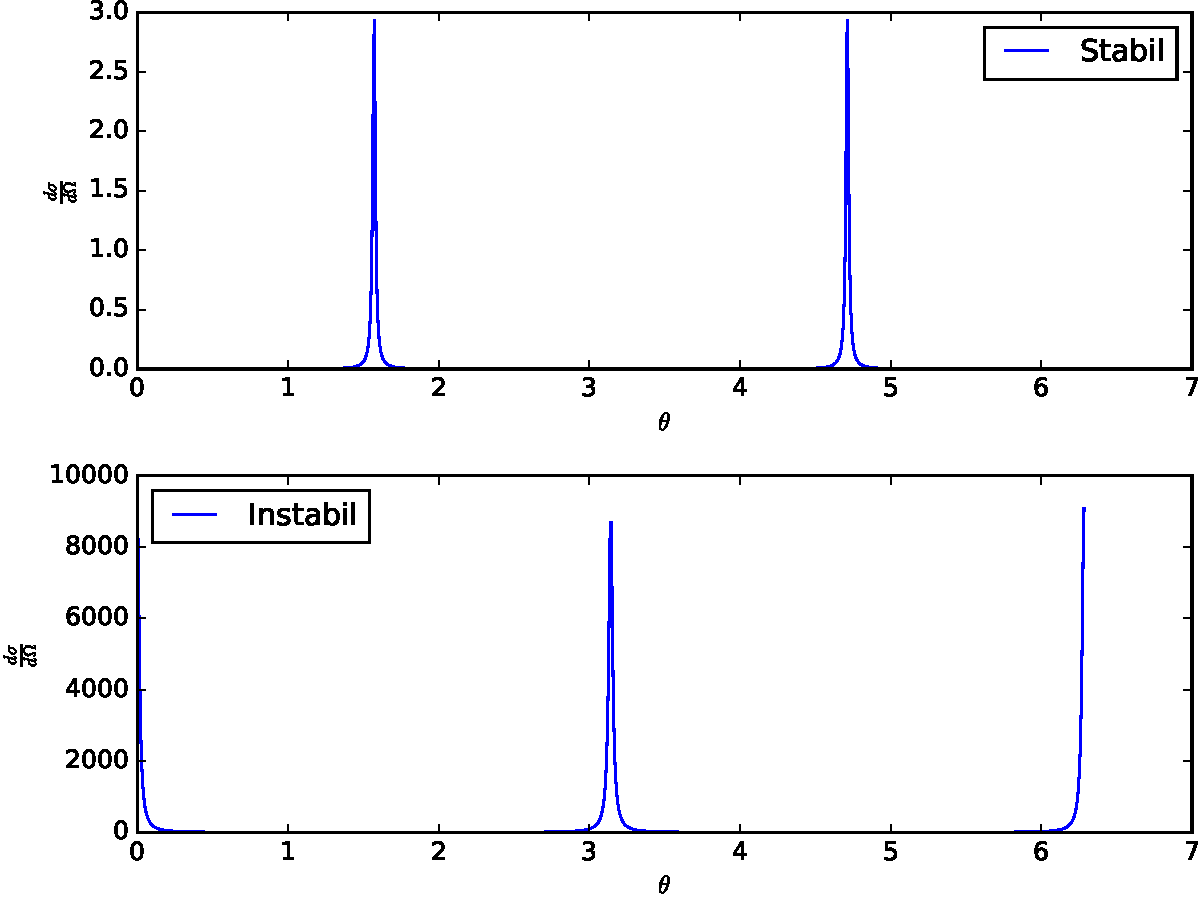
\includegraphics[width=\textwidth]{plots/Stabiplot.pdf}
  \caption{Gegenüberstellung der Stabilität der ursprünglichen und umgeformten Gleichung.}
  \label{fig:gegenstellung}
\end{figure}
\subsection{Aufgabe 2 d)}
Berechnung der Konditionszahlen
\subsection{AUfgabe 2 e)}
